\chapter{分离学习:分布式深度学习的一种资源节约型模型和数据并行方法}

\section*{摘要}
资源限制、工作量开销、缺乏信任和竞争阻碍了多个机构之间共享原始数据。这导致了用于训练最先进的深度学习模型的数据短缺。分裂学习是一种分布式机器学习的模型和数据并行方法,是克服这些问题的高度资源效率的解决方案。分离式学习通过对传统的深度学习模型架构进行划分,使网络中的一些层对客户是私有的,其余的在服务器上集中共享。这使得分布式机器学习模型的训练不需要任何原始数据的共享,同时减少任何客户端所需的计算或通信量。分离式学习的范式有几种变体,取决于手头正在考虑的具体问题。在本章中,我们将分享执行分割学习的理论、经验和实践方面,以及一些可以根据你选择的应用而选择的变体。

\section{分离学习的介绍}
联合学习是一种数据并行的方法,其中数据是分布式的,而作为训练回合一部分的每个客户端都使用自己的本地数据训练完全相同的模型架构。在现实世界中,服务器可能是一个强大的计算资源,但最终却要进行一个相对简单的计算,即对每个客户端学习的权重进行加权平均。在现实世界中,往往存在着与服务器相比资源相对有限的客户。

分离式学习通过将模型架构分割成不同的层,使每个客户保持权重,直到一个被称为分离层的中间层,从而迎合了这种现实的设置。其余的层都在服务器上保存。

\textbf{优点和局限性。} 这种方法不仅减少了任何客户端要进行的计算工作,而且还减少了分布式训练期间需要发送的通信有效载荷的大小。这是因为它只需要在前向传播步骤中从任何客户端向服务器发送来自一个层(分裂层)的激活信息。同时,在反向传播步骤中,只有一个层(分裂层之后的层)的梯度需要由服务器发送至客户端。在模型性能方面,我们根据经验观察到,SplitNN的收敛速度仍然比联合学习和大批量同步随机梯度下降快得多。也就是说,当在较少的客户上进行训练时,它需要相对较大的整体通信带宽,尽管在有大量客户的情况下,它最终比其他方法低得多。先进的神经网络压缩方法,如,可以用来减少通信负荷。通信带宽也可以通过允许在客户端有更多的层来表示进一步压缩的表征来换取客户端的计算。

在分割学习中共享中间层的激活也与局部并行[8]、特征重放[9]和分割征服量化[10]的分布式学习方法有关。这是与联合学习中的权重共享相对应的。

\subsection{普通的分离学习}
在这种方法中,每个客户端训练网络到某一层,即分裂层,并将权重发送到服务器(图19.1)。然后服务器训练网络的其他层。这就完成了前向传播的过程。然后,服务器为最后一层生成梯度,并反向传播错误,直到分裂层。
然后,梯度被传递给客户端。其余的反向传播由客户端完成。这样一直持续到网络训练完成。分割的形状可以是任意的,不一定是垂直的。在这个框架中,也没有明确的原始数据的共享。
\begin{figure}
	\centering
	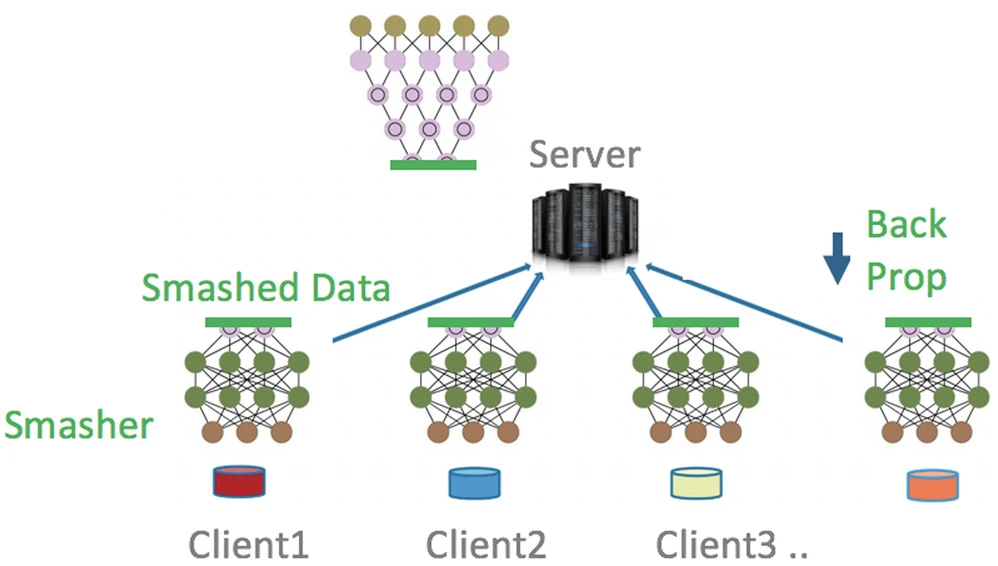
\includegraphics[width=0.8\textwidth]{chapter19/images/Fig.19.1}
	\caption{有多个客户端和一个服务器的分割学习设置,绿色虚线显示了客户端的层份额和服务器的层份额之间的分割。在前向传播过程中,只有分割层(客户的最后一层)的激活被共享,在反向传播过程中,只有服务器的第一层的梯度与客户共享。} \label{fig:19.1}
\end{figure}

\subsubsection{同步步骤}
在每个客户端完成其历时后,下一个排队完成其历时的客户端会收到来自前一个客户端的本地权重(直到分割层的权重)作为其历时的初始化。

\subsubsection{放宽同步要求}
客户端之间的这种额外的通信可以通过像BlindLearning[11]这样的分割学习方法来避免,该方法基于使用一个损失函数,该函数是每个客户端完成的前向传播获得的损失的平均值。同样,通过splitFedv1[12]、splitFedv2[12]和splitFedv3[13]进一步减少了通信和同步要求,这些都是分割学习和联合学习的混合方法。在[14]中提供了一种改善延迟的混合方法。

 \section{通信效率[15]}
在这一节中,我们描述了我们对分割学习和联合学习这两种分布式学习设置的通信效率的计算。为了分析通信效率,我们考虑了每个客户端为训练和客户端权重同步所传输的数据量,因为影响通信速率的其他因素取决于训练集群的设置,而与分布式学习设置无关。我们使用以下符号来数学地衡量通信效率。

\textbf{符号} $K=\#$客户,$N=\#$模型参数,$p=$总数据集大小,$q=$分割层大小,$\eta=$客户的模型参数(权重)的比例,因此$1-\eta$是服务器的参数比例。

在表19.1中,我们显示了每个客户端在一个历时中所需要的通信,以及所有客户端在一个历时中所需要的总通信。由于有$K$个客户端,当每个客户端的训练数据集的大小相同时在分割学习中,每个客户会有$p/K$的数据记录。因此,在前向传播过程中,分裂学习中每个客户端传递的激活大小为$(p/K)q$,在后向传播过程中,每个客户端传递的梯度大小也为$(p/K)q$。在有客户端权重共享的虚无分裂学习情况下,将权重传递给下一个客户端将涉及ηN的通信。在联合学习中,在上传单个客户端权重和下载平均权重的过程中,权重/梯度的通信都是$\eta N$。平均值的过程中,权重/梯度的通信量都是$N$的大小。

\section{延迟}
根据客户端和服务器的计算能力限制,计算的延迟需要最小化,同时保持高的通信效率。为此,[14]对普通分割学习、splitFed和[14]中提出的方法的延迟进行了分析比较。他们考虑了以下模型大小的符号

\section{分离学习的拓扑结构}
\subsection{多样化的配置}
除了所讨论的普通式分离学习及其需要较少同步的变体外,还有其他可以使用分离学习的拓扑结构,如下文所述。
\begin{figure}
	\centering
	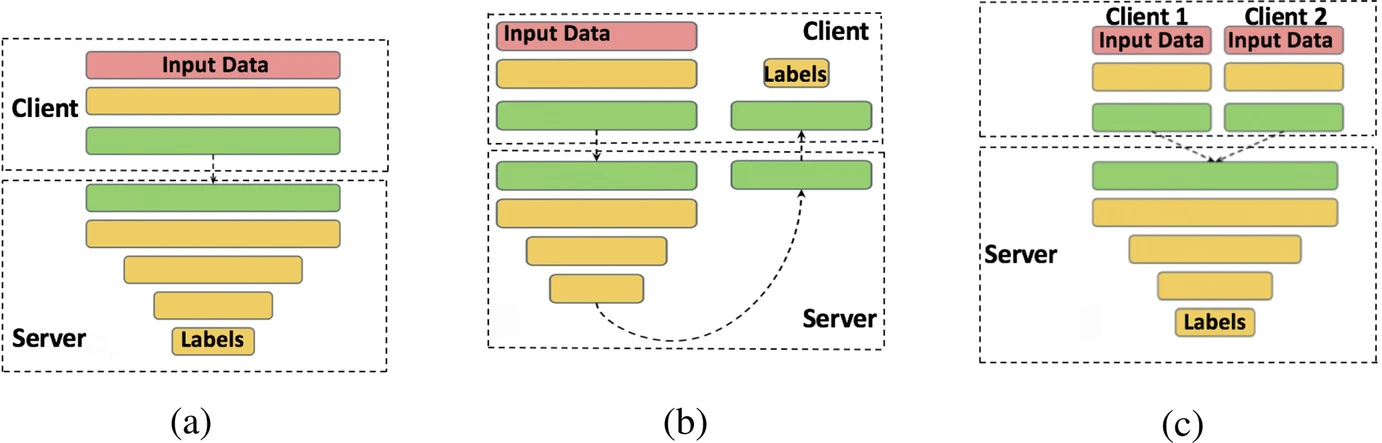
\includegraphics[width=0.8\textwidth]{chapter19/images/Fig.19.2}
	\caption{健康的分割学习配置显示原始数据不在客户端和服务器健康实体之间传输,用于用SplitNN对分布式深度学习模型进行训练和推理。(a) 简单的香草式分割学习。(b) 没有标签共享的分割学习。(c) 纵向分割数据的分割学习} \label{fig:19.2}
\end{figure}

\begin{enumerate}
	\item \textbf{无标签共享的分割学习的U型配置[3] [16]:}本节描述的另外两种配置涉及到标签的共享,尽管它们彼此之间不共享任何原始输入数据。我们可以通过一个不需要客户共享任何标签的U型配置来完全缓解这个问题。在这个设置中,我们在服务器网络的末端层将网络包裹起来,并将输出送回客户实体,如图19.2b所示。虽然服务器仍然保留着它的大部分层,但客户端从末端层产生梯度,并将其用于反向传播,而不共享相应的标签。在标签包括高度敏感信息的情况下,如病人的疾病状况,这种设置是分布式深度学习的理想选择。
	\item \textbf{分割学习的垂直分区数据[17]:}这种配置允许持有不同模式的病人数据的多个机构学习分布式模型,而无需共享数据。在图19.2c中,我们展示了一个适合这种多模式多机构合作的SplitNN的配置实例。作为一个具体的例子,我们介绍了放射科中心与病理测试中心和疾病诊断的服务器合作的情况。如图19.2c所示,持有成像数据模式的放射科中心训练一个部分模型,直到分裂层。以同样的方式,拥有病人测试结果的病理测试中心训练一个部分模型,直到它自己的分割层。然后,来自这两个中心的分割层的输出被串联起来,并被发送到疾病诊断服务器,以训练模型的其余部分。这个过程来回继续,完成前向和后向传播,以训练分布式深度学习模型,而不分享彼此的原始数据。
	\item \textbf{扩展的香草分割学习:}如图19.3a所示,我们给出了香草分割学习的另一个修改方案,即连接输出的结果在传递给服务器之前在另一个客户端进一步处理。
	\item \textbf{多任务分割学习的配置:}如图19.3b所示,在这个配置中,来自不同客户的多模式数据被用来训练部分网络,直到其相应的分割层。每个分割层的输出都被串联起来,然后发送到多个服务器。每个服务器使用这些数据来训练多个模型,以解决不同的监督学习任务。
	\item \textbf{类似Tor[18]的配置,用于多跳分割学习:}这种配置是vanilla配置的一个类似的扩展。在这种情况下,多个客户端依次训练部分网络,每个客户端最多训练一个分割层,并将其输出转移到下一个客户端。这个过程继续进行,如图19.3c所示,最终客户将其激活从其分割层发送到服务器以完成训练。
\end{enumerate}
\begin{figure}
	\centering
	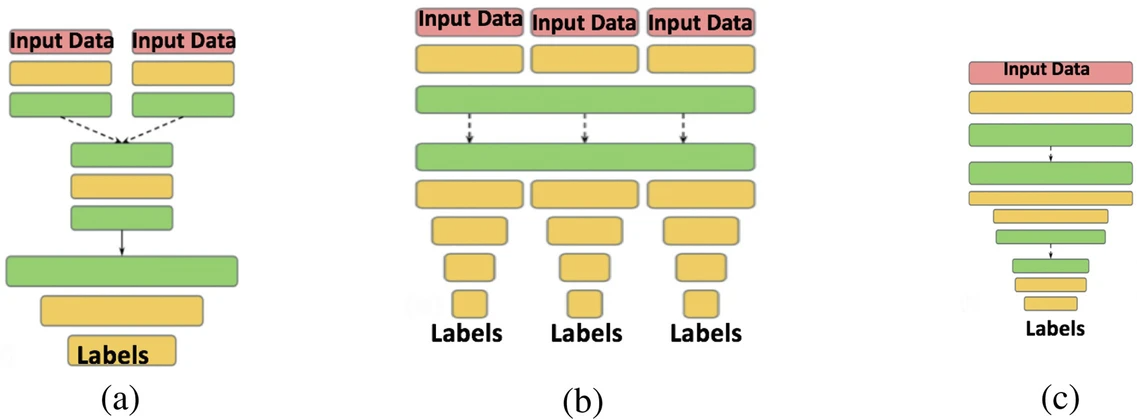
\includegraphics[width=0.8\textwidth]{chapter19/images/Fig.19.3}
	\caption{健康的分割学习配置显示原始数据不在客户端和服务器健康实体之间传输,用于用SplitNN进行分布式深度学习模型的训练和推理。(a) 扩展的香草。 (b) 垂直分割输入的多任务输出。(c) 'Tor' [18]} \label{fig:19.3}
\end{figure}

我们想指出的是,尽管这些例子的配置显示了SplitNN的一些多功能应用,但它们绝不是唯一可能的配置。

\subsection{用ExpertMatcher选择模型[19]}
在某些情况下,一个强大的服务器托管着多个专有模型的存储库,它希望通过预测API在机器学习即服务(MLaaS)的商业模式中使用。这些专有模型不能被提供给客户下载。同时,客户往往有敏感的数据集,它希望获得预测结果。在这种情况下,出现了一个问题,即如何从服务器的存储库中找到与客户持有的数据集相匹配的正确模型。ExpertMatcher就是这样一个基于U型回旋镖分割学习拓扑结构的模型选择架构。

\subsection{实现细节}
我们假设在集中式服务器上有$K$个预训练的专家网络,每个网络都有其相应的预训练的无监督表征学习模型(本例中我们考虑自动编码器(AE))$\phi_{K}$在特定任务的数据集上训练过。考虑到AE所训练的数据集,我们提取整个数据集的编码表征,并计算出数据集的平均表征$\mu_{k} \in \mathbb{R}{d}, k \in \left\{ 1, \cdots, K \right\}$,其中$d$是特征维度。假设数据集由$N$个对象类别组成,我们也计算出数据集中每个类别的平均代表性$\mu_{k}{n} \in \mathbb{R}^{d}, n \in \left\{ 1, \cdots, N \right\}, k \in \left\{ 1, \cdots, K \right\}$。

客户端(客户A和客户B)利用与服务器类似的方法,客户为每个$p$和$q$的数据集训练他们独特的AE,客户A:$p \in \left\{ 1,\cdots, P \right\}$和客户端B:$q \in \left\{ 1,\cdots, Q \right\}$。 让我们假设对于客户A来说,从隐藏层提取的样本$X^1_p$的中间特征给定为$x^1_p = \phi^1_p(X^1_p)$,同样,对于客户B来说,它是$x^2_q = \phi^2_q(X^2_q)$。为了简洁起见,我们把来自任何客户端的中间表征表示为$x^{'}$。

我们首先要解释一下标签的粗细概念,我们的意思是,数据中的类是由高层次(粗)或低层次(细)的语义类别分开的。举例来说,把狗和猫分开的类是粗的类别,而把不同类型的狗分开的类是细的类别。在ExpertMatcher的概念中,对于客户数据的粗放式分配(CA)。对于编码后的表示$x^{'}$,我们分配一个服务器AE,$k^{*} \in \left\{ 1, \cdots, K \right\}$,该服务器与$x^{'}$具有最大的相似度$\mu_{k}$;见图19.4。
\begin{figure}
	\centering
	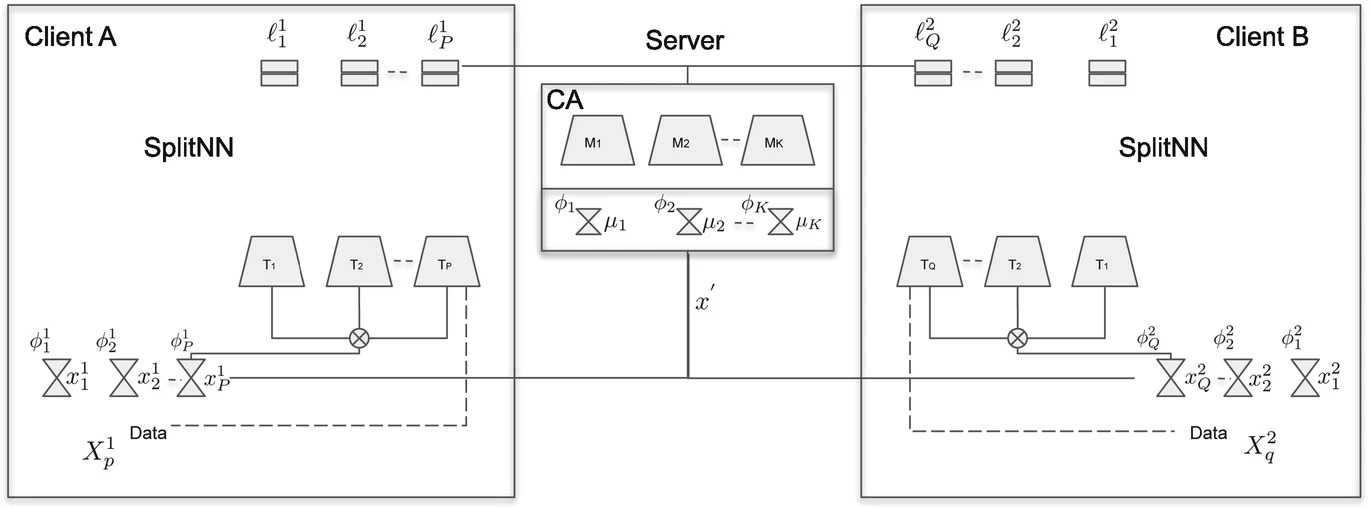
\includegraphics[width=0.8\textwidth]{chapter19/images/Fig.19.4}
	\caption{pass} \label{fig:19.4}
\end{figure}

对于客户数据的细粒度(FA)分配:对于编码后的表示$x^{'}$,我们分配一个专家网络$M_{n},n \in \left\{ 1, \cdots,N \right\}$,该网络具有$x^{'}_{k^{*}}$与$\mu^{n}_{k}$的最大相似度。用于分配的相似性的选择取决于用户。余弦相似性、距离相关性、信息论测量、希尔伯特-施密特独立准则、最大平均差异、内核目标对齐和积分概率指标只是相似性指标的几种可能性。

最后在给定的样本分配到模型后,人们可以很容易地训练一个SplitNN类型的架构[3]。

在目前的设置中,由于服务器不能接触到客户的原始数据,而是一个非常低维的编码表示,因此保留了一个弱水平的隐私。

请注意,这种方法有一个不足之处。如果服务器没有专门用于客户数据的AE模型,客户数据就会因为最大余弦相似性准则而发生错误分配--这可以通过在服务器上增加一个额外的模型来解决,该模型执行二元分类:客户数据与服务器数据匹配或不匹配。

\section{分离学习的协作推理}
由于企业能够利用大规模的计算资源在巨大的数据集上训练超大型机器学习模型,这为打算用这些模型进行预测的外部客户带来了一系列新的问题。鉴于这些大型模型通常有数十亿个参数,客户不愿意在设备上完整地下载这些模型。使用这些模型进行预测,仅在设备上进行计算资源密集。这就开启了私人协作推理(PCI)的问题,在这个问题上,模型被分割到客户端和服务器上(表19.3)。

客户的数据是私有的,因此在这种情况下交流的激活需要被正式私有化,以防止成员推理和重建攻击。在另一种情况下,服务器打算私下分享训练好的模型的权重,这类工作已经相当多了。在这种PCI的设置中,考虑的隐私是关于服务器自己的数据的。而PCI的设置是相对较新的,因为它要求在私人推理期间对客户自己的私人数据进行私人共享激活,而不是在私人训练后对服务器的数据进行私人共享权重。这需要在基于激活共享而非权重共享的分布式机器学习和正式隐私的交叉点上进行创新。

\subsection{防止协作推理中的重构攻击}
需要获得预测的客户的数据记录是私有的,因此,在这种PCI设置中交流的模型的中间表征(或激活)需要被脱敏,以防止重建攻击(图19.5)。从架构的角度来看,保护隐私的机器学习还没有达到其AlexNet时刻。该领域在DP-SGD[24]及其变体等正式的隐私机制方面取得了快速的进展。在这些方法中,仍然有很大的空间来改进目前的隐私与效用的权衡,使其适用于许多生产用例。我们现在描述激活共享方面的一些进展,用于(a)防止训练数据方面的成员推理攻击和(b)防止PCI设置中的预测查询数据的重建攻击。
\begin{figure}
	\centering
	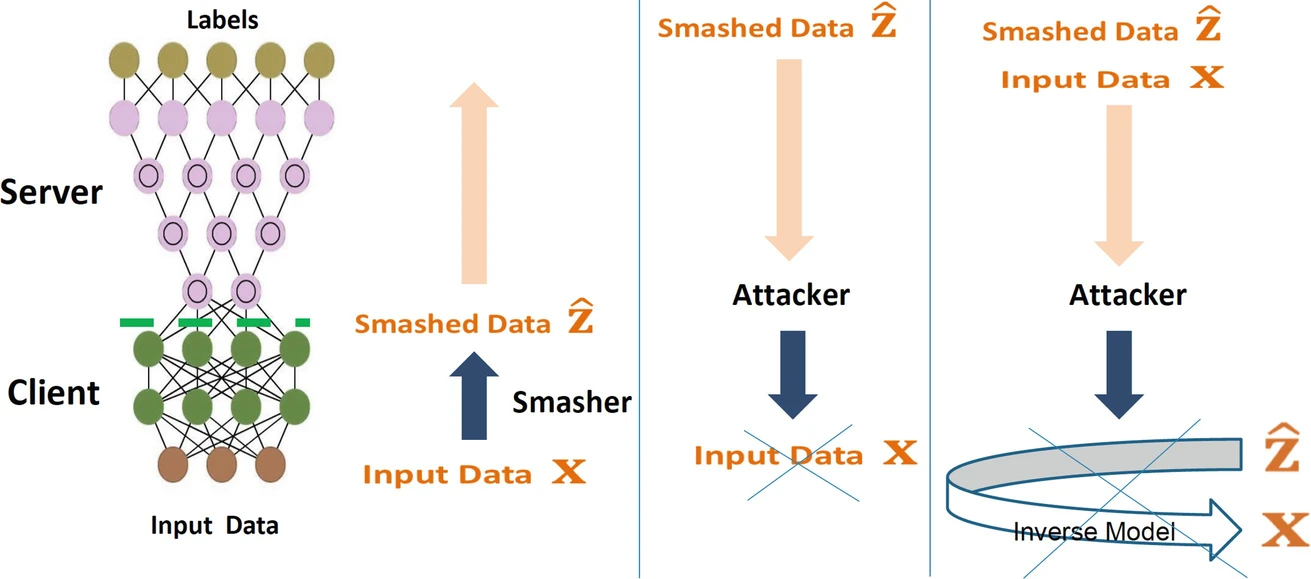
\includegraphics[width=0.8\textwidth]{chapter19/images/Fig.19.5}
	\caption{pass} \label{fig:19.5}
\end{figure}

\subsubsection{信道剪枝}
[20]中的工作表明,学习一个修剪滤波器来选择性地修剪掉分裂层潜伏表征空间中的通道,有助于在PCI设置的预测步骤中凭经验防止各种先进的重建攻击(图19.6)。
\begin{figure}
	\centering
	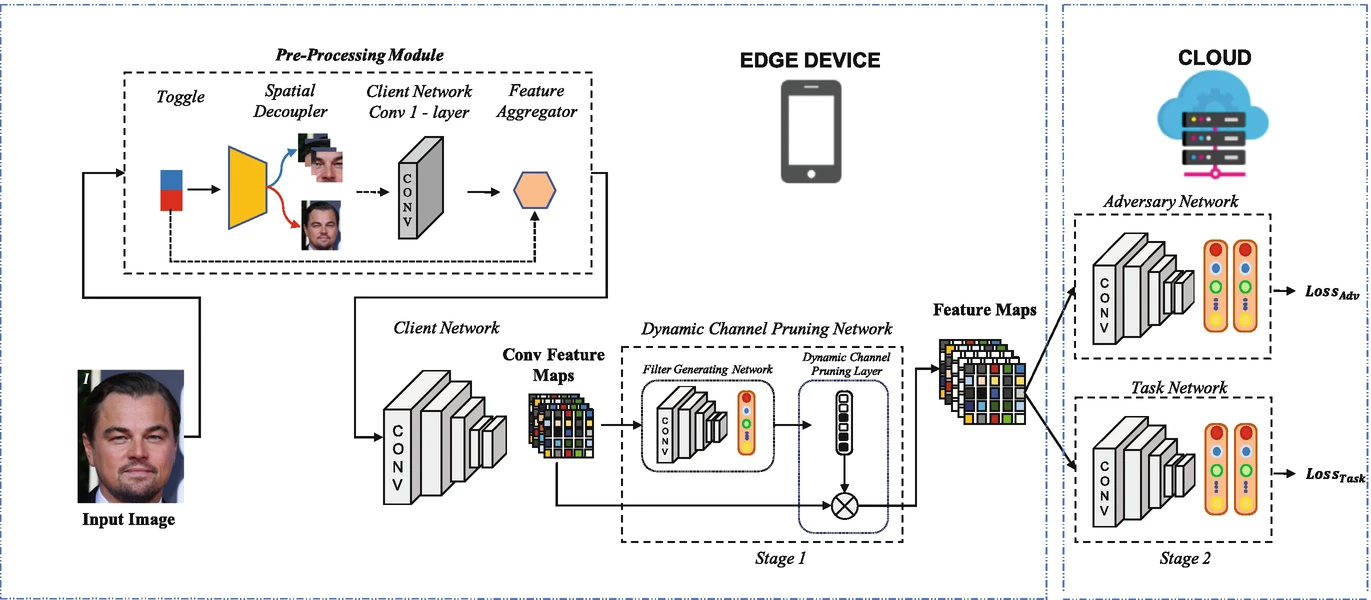
\includegraphics[width=0.8\textwidth]{chapter19/images/Fig.19.6}
	\caption{pass} \label{fig:19.6}
\end{figure}
**图 19.6** 参考文献[20]显示,学习一个修剪滤波器来选择性地修剪掉分裂层潜伏表征空间中的通道,有助于在PCI设置的预测步骤中凭经验防止各种最先进的重建攻击。

\subsubsection{相关性}
这里的关键思想是通过在常用的分类损失项--分类交叉熵上增加一个额外的损失项来减少信息泄露。我们使用的减少信息泄漏的损失项是距离相关,这是随机变量之间非线性(和线性)统计依赖性的有力措施。距离相关损失在原始输入数据和任何选定的层的输出之间最小化,这些层的输出需要从客户端传达给另一个不受信任的客户端或不受信任的服务器。这种设置对一些流行的分布式机器学习形式至关重要,这些机器学习需要共享中间层的激活。这已经在动机部分的 "激活共享 "小节中得到了激励。

这种损失组合的优化有助于确保由保护层产生的激活有最小的信息来重建原始数据,同时在后处理时仍有足够的作用来达到合理的分类精度。实验部分从质量和数量上证实了在保持合理分类精度的同时防止重建原始输入数据的质量。距离相关性与交叉熵的联合最小化导致了一种专门的特征提取或转换,从而使其在人类视觉系统和更复杂的重建攻击方面无法察觉原始数据集的信息泄露。

\subsubsection{损失函数}
输入数据$X$的$n$个样本、保护层$Z$的激活、真实标签$Y_{true}$、预测标签$Y$和标量权重$\alpha$的总损失函数由以下公式给出:
\begin{align}
	\alpha DCOR(X, Z) + (1 - \alpha) CCE(Y_{true}, Y)
\end{align}

\subsection{激活共享的差异性隐私}
Arachchige等人[21]提供了一个差分隐隐私机制,用于分享卷积层和池化层之后得到的扁平化层的激活值。这些扁平化的输出被二进制化,一个受RAPPOR启发的 "效用增强的随机化 "机制被应用来创建一个差分隐私的二进制表示。然后,这些数据被传送到服务器,在那里全连接层对它们进行操作以产生最终的预测结果。[22]中的工作为从深度网络中提取的特征的监督流形嵌入提供了一种差分隐私机制,以便从服务器上的数据库执行图像检索任务。[23]的工作着眼于防止在分离学习的背景下标签信息的泄漏。它们提供了防止规范和暗示攻击泄露标签信息的防御措施。

\section{未来工作}
关于分布式机器学习方法,如分离学习和联邦学习,有几个方面需要研究。这些问题包括资源效率、隐私、收敛性、现实世界数据的非均匀性、训练的延迟、协作推理、滞后的客户端、通信的拓扑结构、攻击测试平台等等,使这一领域成为当前研究的活跃领域。
